\section{The first-generation strategy and what it left unsolved}\label{sec:rtb}

\para{Design:} The score is an equal-weight composite of 63-session breadth, event-day breadth and momentum-orthogonal breadth. The book holds the top three names long and the bottom three short, rebalances weekly with hysteresis, and weights each leg by inverse GJR-GARCH-t volatility. The tilt sets the leg budgets to $\pm0.25$ when a forward-filtered two-state hidden Markov model is in the calm state and the equal-weight index is above its 200-day average.

\para{What it solved:} Most of the infrastructure used later in the paper comes from RTB. Target snapshots carry knowledge dates, cleaning is logged, truncation tests run on every feature, risk models are walk-forward, the specification is frozen before evaluation, and the backtest is vectorised. In development RTB had a CAGR of 16.6\%, a Sharpe ratio of 1.56 and a Calmar ratio of 1.77.

\para{What it did not solve:} Figure~\ref{fig:camouflage} decomposes RTB
\begin{itemize}
  \item \emph{Timing:} The timing leg earns 11.0\% a year at a Sharpe ratio of 1.69. Its average net exposure is $+0.35$, and a static exposure of that size (0.35 times the market) ends above the timing leg. Treynor-Mazuy and Henriksson-Merton regressions show no timing ability
  \item \emph{Selection:} In DEV the selection leg has a Sharpe ratio of 0.63 and a Calmar ratio of 0.36
  \item \emph{Signal:} The breadth features have rank correlations of 0.55-0.78 with price momentum
\end{itemize}
In the terms of Section~\ref{sec:framework}, RTB's Calmar ratio was camouflaged beta on a selection signal that behaved much like momentum.

\begin{figure}[t]
\centering
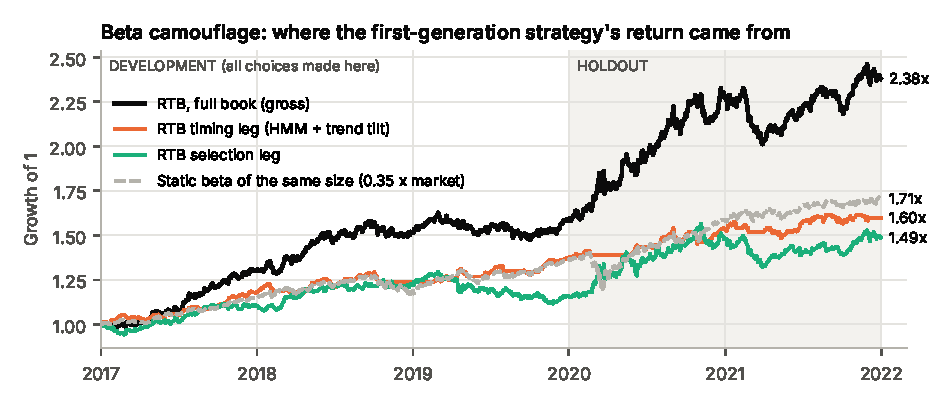
\includegraphics[width=\figw]{fig/fig01.pdf}
\caption{Beta camouflage in the first-generation strategy (RTB). Cumulative gross returns of the full book, of its timing leg (the hidden-Markov and trend tilt of the leg budgets), of its dollar-neutral selection leg, and of a static market exposure equal to the book's average net exposure (0.35). The static exposure finishes above the timing leg, so the overlay delivered the equity premium of the sample and no timing skill.}\label{fig:camouflage}
\end{figure}

\para{The search that followed:} Six audit rounds then looked for a selection alpha, with every new family of hypotheses pre-registered (Table~\ref{tab:ledger}). None of the following passed its pre-registered tests:
\begin{itemize}
  \item new analyst features, an extended library of 18 signals and signal blends
  \item analyst-network spillovers, idiosyncratic momentum and a L\'evy-area lead--lag signal
  \item event-level post-revision drift, analyst-skill weighting and earnings-cycle conditioning
  \item within-analyst relative valuation, normalised revision velocity and dispersion gating
  \item earnings-reaction predictability, and risk-forecasting overlays (Round 6)
\end{itemize}
These rounds taught me two things. Cutting the sample into subsets (event days, analyst histories, cycle phases) lost more power in breadth than it gained in precision, and level signals on target prices carry the price in their denominator. What I needed next was a selection signal with information beyond price momentum, in a construction with no beta.

\begin{table}[t]
\centering\footnotesize
\caption{Research ledger: hypotheses tested before and around the final specification}\label{tab:ledger}
\begin{adjustbox}{max width=\textwidth}\begin{tabular}{p{0.07\textwidth}p{0.43\textwidth}p{0.42\textwidth}}
\toprule
Round & Hypotheses / signals & Outcome\\
\midrule
1 & Fresh-vs-stale consensus wedge, leader/laggard revisions, conviction shock (target change net of price change), post-event drift, bold-revision breadth, peer spillover, quarterly target expiry & None passed the inclusion rule, strongest (conviction shock) IC21 0.034, $p = 0.30$, a 252-session expiry is retained.\\
2 & Library of 18 signals (11 analyst, 7 price), four pre-specified blends, analyst window, rebalancing frequency & LMH is the only signal with FM $t > 2$, blends do not improve, flow window 63 sessions, slower rebalancing dominates.\\
3 & Analyst-network pending revisions (2), idiosyncratic momentum, L\'evy-area lead--lag, upside per unit of volatility, tranche period, volatility scaling & 0 of 10 significant after Holm, network signals wrong-signed, slow tranches, volatility scaling hurts.\\
4 & Eight pre-registered tests: event-level LMH, post-revision drift, confirmed surprise, analyst-skill persistence, two skill-weighted breadths, earnings-phase interaction and gating, overlay decomposition & 0 of 8 after Holm, skill does not persist ($t = -0.22$), event drift reverses in DEV but not in a one-shot holdout test, the overlay is beta.\\
5 & Within-analyst demeaned and ranked target returns, top-pick-weighted breadth, normalised revision velocity (2), dispersion-gated breadth, quiet-day breadth, coverage change, breadth acceleration, linear-rank weights & 0 of 9, within-analyst valuation wrong-signed (IC21 $-0.089$), flow variants duplicate breadth (correlation 0.86--0.96), linear-rank weights worse.\\
6 & Feasibility, persistence-preserving placebos, signal decomposition, earnings-reaction predictability, variance forecasting, risk-based sizing & Reaction predictability null in DEV, analyst dispersion and an earnings-calendar proxy forecast variance beyond GARCH, but sizing by them does not improve the book.\\
\bottomrule
\end{tabular}\end{adjustbox}
\par\smallskip\begin{minipage}{0.95\textwidth}\footnotesize The audit also found and corrected a construction error: a rank-proportional book that was not dollar-neutral (a cross-sectional rank centred at $0.5/N$ instead of zero), which its beta and its random-score placebo exposed.\end{minipage}
\end{table}
